\documentclass[a4paper,twocolumn,11pt,nopdfoutputerror]{quantumarticle}
\usepackage[utf8]{inputenc}
\usepackage[T1]{fontenc}
\usepackage[english]{babel}
\usepackage{amsmath,amssymb,amsthm,mathtools}
\usepackage{braket}
\usepackage{graphicx}
\usepackage{booktabs}
\usepackage{siunitx}
\usepackage{microtype}
\usepackage{xcolor}
\usepackage[numbers,sort&compress]{natbib}
\usepackage[ruled,vlined]{algorithm2e}
\usepackage{enumitem}
\usepackage{multirow}
\usepackage{bbm}
\usepackage{makecell}

% ---------- macros ----------
\DeclareMathOperator{\Tr}{Tr}
\newcommand{\F}{\mathbb{F}}
\newcommand{\R}{\mathbb{R}}
\newcommand{\Pauli}{\mathcal{P}}
\newcommand{\synd}{\mathbf{s}}
\newcommand{\err}{\mathbf{e}}
\newcommand{\ehat}{\hat{\mathbf{e}}}
\newcommand{\llr}{\Lambda}
\newcommand{\Hmat}{\mathbf{H}}
\newcommand{\Gmat}{\mathbf{G}}
\newcommand{\Wmat}{\mathbf{W}}
\newcommand{\bvec}[1]{\mathbf{#1}}
\newcommand{\phat}{\hat{p}}
\newcommand{\concat}{\,\|\,}
\newcommand{\code}[3]{\ensuremath{[\![#1,#2,#3]\!]}}
\newcommand{\pending}[1]{\textcolor{red}{\textbf{[#1]}}}
\newtheorem{proposition}{Proposition}
\newtheorem{remark}{Remark}

\graphicspath{{./figures/}{./}}
\DeclareGraphicsExtensions{.pdf,.png,.jpg}

\usepackage{hyperref}
\hypersetup{colorlinks=true,citecolor=blue,linkcolor=blue,urlcolor=blue}

% ============================================================
%  TITLE
% ============================================================
\title{GNN-Augmented Belief Propagation for Bivariate Bicycle Codes: Gains, Baseline Sensitivity, and Calibration Side Information}

\author{Jothiradithya Sai Konduru}
\affiliation{Paradise Valley High School, Phoenix, AZ, USA}

\author{Anish Chedalla}
\affiliation{Paradise Valley High School, Phoenix, AZ, USA}

\author{Nithin Raveendran}
\affiliation{Department of Electrical and Computer Engineering,
             University of Arizona, Tucson, AZ, USA}
\email{nithin@arizona.edu}


\begin{document}
\maketitle

% ============================================================
%  ABSTRACT
% ============================================================
\begin{abstract}
Bivariate bicycle (BB) quantum low-density parity-check (QLDPC) codes
combine finite encoding rate with low-weight checks, but their loopy
Tanner graphs remain challenging for iterative decoding. Learned
message-passing can improve belief propagation (BP), although the
measured gain depends strongly on the BP configuration used for
training and evaluation. We study this issue using a Tanner-graph
neural network (\textsc{TannerGNN}) that produces qubit-wise log-likelihood
corrections for BP under a biased CSS component-noise model. On the
$\code{72}{12}{6}$ BB code, a model trained with 10-iteration flooding
BP reduces the logical error rate (LER) from $0.0990$ to $0.0838$ on
8{,}000 held-out syndromes at $p=0.04$ and $\eta=20$, a $15.4\%$
relative reduction (paired McNemar $p<10^{-15}$). This gain does not
transfer to a stronger serial min-sum BP-OSD decoder: the learned
correction is statistically indistinguishable at lower tested error
rates and degrades performance at $p\geq 0.04$. Independent baseline
experiments further show that schedule, BP update rule, iteration count,
and OSD configuration can change LER by orders of magnitude. These
settings must therefore be specified and controlled when learned decoders
are compared.
We also establish that unclipped min-sum BP is invariant, in its hard
decisions, to a uniform positive rescaling of all channel LLRs within a
CSS component. Thus, changing only the magnitude of a uniform prior
cannot make the underlying min-sum BP adaptive, although a learned
network may still use global context through other pathways. Finally,
synthetic experiments with heterogeneous per-qubit error rates show a
large gap between mean-prior and oracle-prior decoding, motivating
spatially resolved calibration side information rather than a single
global noise scalar. The experiments show that an improvement over one BP baseline does not
by itself establish an improvement over a stronger decoder, and that
spatial calibration information is qualitatively different from a single
global noise estimate.
\end{abstract}

% ============================================================
%  I. INTRODUCTION
% ============================================================
\section{Introduction}

Bivariate bicycle (BB) codes provide a concrete finite-length setting in
which QLDPC codes combine non-vanishing encoding rate, weight-six
stabilizer checks, and syndrome-extraction circuits compatible with
low-degree connectivity~\cite{Bravyi2024Memory}. IBM's current
fault-tolerant architecture is explicitly based on BB codes, making the
finite-length decoding behavior of this family practically relevant as
well as theoretically interesting~\cite{IBMRoadmap2025}. The canonical
examples include the $\code{72}{12}{6}$, $\code{144}{12}{12}$, and
$\code{288}{12}{18}$ codes studied here.

The decoding bottleneck is not the absence of efficient iterative
algorithms, but their finite-length failure modes. BP is attractive
because its message updates are local and parallelizable, yet short
cycles and degeneracy in QLDPC Tanner graphs create correlated messages
and non-convergent or incorrect fixed points~\cite{Roffe2020Landscape}.
OSD post-processing can recover many BP failures, while recent learned
decoders use graph neural networks (GNNs) either to replace BP or to
intervene between BP stages~\cite{Gong2024GNN,Maan2025MLBP}. These
approaches make the choice of baseline unusually consequential: a neural
correction trained against one BP schedule or stopping rule need not
address the residual failures of a stronger decoder.

A second issue is adaptivity. Hardware noise is neither spatially nor
temporally uniform, and calibration information can therefore be useful
to a decoder. However, three distinct sources of information should not
be conflated: a global estimate of the physical error rate, spatially
resolved per-qubit calibration data, and syndrome history. A decoder may
respond differently to each. In particular, changing the magnitude of a
uniform channel prior has a restricted effect on min-sum BP, whereas
per-qubit priors can change the relative reliability ordering that drives
both BP and OSD.

We study a GNN-augmented BP pipeline with two questions in view:
\emph{what gain does the learned correction provide relative to the BP
decoder used in training, and what additional information is needed for
noise adaptation?} We compare decoder configurations, training and
evaluation baselines, and different forms of calibration information to
isolate the source of the observed performance changes.

\subsection{Contributions}\label{sec:contributions}

Our main findings are:
\begin{enumerate}[leftmargin=*,topsep=3pt,itemsep=3pt]
\item \textbf{A held-out GNN gain over its training-aligned BP baseline.}
On $\code{72}{12}{6}$ at $p=0.04$ and $\eta=20$,
\textsc{TannerGNN}+flooding BP reduces LER from $0.0990$ to $0.0838$
on 8{,}000 held-out syndromes, corresponding to a $15.4\%$ relative
reduction (McNemar $p<10^{-15}$). The model is trained only on
$p\in[0.02,0.03]$, so this test is also outside the training error-rate
range (Sec.~\ref{sec:gnn_positive}).

\item \textbf{Baseline configuration and alignment can dominate the
apparent learned gain.} Serial min-sum BP with OSD post-processing is
substantially stronger than the flooding BP used in GNN training. The
same learned correction does not improve this stronger decoder and is
worse at the two highest tested error rates. Separate experiments on
$\code{288}{12}{18}$ show order-of-magnitude sensitivity to BP schedule,
update rule, iteration count, and OSD settings. The
training decoder and evaluation decoder are therefore part of the
experimental condition rather than interchangeable implementations of
``BP''
(Secs.~\ref{sec:baseline} and~\ref{sec:mismatch}).

\item \textbf{Global prior scaling and spatial calibration carry
different information.} We prove that hard decisions of unclipped
min-sum BP are invariant to a uniform positive rescaling of the channel
LLRs within a CSS component. This result limits adaptivity obtained only
by changing a uniform BP prior; it does not rule out a learned network
using a global noise scalar as context. In synthetic heterogeneous-noise
experiments, providing the true per-qubit rates to BP-OSD yields large
oracle improvements, motivating spatially resolved calibration inputs.
Because code size and operating point co-vary in these experiments, we do
not attribute the cross-code trend to distance alone
(Secs.~\ref{sec:invariance} and~\ref{sec:oraclegap}).
\end{enumerate}
\section{Background}\label{sec:background}

\subsection{CSS codes and bivariate bicycle construction}

A CSS code~\cite{Calderbank1996Good,Steane1996Error} is defined by
matrices $\Hmat_x, \Hmat_z \in \F_2^{m \times n}$ with
$\Hmat_x \Hmat_z^\top = \mathbf{0}$. The syndrome of an error
$(e_x, e_z)$ decomposes as
$s_x = \Hmat_x e_z$,
$s_z = \Hmat_z e_x$
over $\F_2$, so $X$- and $Z$-type errors are decoded independently.
This CSS independence is structurally important for the results
of Sec.~\ref{sec:invariance}.

Bivariate bicycle codes~\cite{Bravyi2024Memory} are constructed
over the group algebra $\F_2[x,y]/(x^\ell-1,\,y^m-1)$. Polynomials
$A(x,y)$ and $B(x,y)$ yield circulant block matrices:
\begin{equation}
\Hmat_x = [\mathbf{A} \mid \mathbf{B}], \qquad
\Hmat_z = [\mathbf{B}^\top \mid \mathbf{A}^\top].
\label{eq:bb}
\end{equation}
We study three codes (Table~\ref{tab:codes}).

\begin{table}[t]
\centering
\small
\caption{Bivariate bicycle codes studied in this work, with
         generator polynomials from \cite{Bravyi2024Memory}.}
\label{tab:codes}
\begin{tabular}{@{}lcccccc@{}}
\toprule
Code & $n$ & $k$ & $d$ & Rate & $\ell$ & $m$ \\
\midrule
$\code{72}{12}{6}$   &  72 & 12 &  6 & 1/6  &  6 &  6 \\
$\code{144}{12}{12}$ & 144 & 12 & 12 & 1/12 & 12 &  6 \\
$\code{288}{12}{18}$ & 288 & 12 & 18 & 1/24 & 12 & 12 \\
\bottomrule
\end{tabular}
\end{table}

\subsection{Belief propagation and its failure modes}\label{sec:bp}

Min-sum BP on a CSS Tanner graph iterates variable-to-check and
check-to-variable messages for $T$ steps. For a check $c_j$ with measured
syndrome bit $s_j$ and a neighboring variable $v_i$,
\begin{align}
\mu_{v_i \to c_j}^{(t)}
&= \llr_i + \!\!\sum_{j' \in \mathcal{N}(i)\setminus j}\!\!
\mu_{c_{j'} \to v_i}^{(t-1)},
\label{eq:vtc}\\
\mu_{c_j \to v_i}^{(t)}
&= (-1)^{s_j}
\!\!\prod_{i' \in \mathcal{N}(j)\setminus i}\!\!
\mathrm{sgn}\!\left(\mu_{v_{i'}\to c_j}^{(t)}\right) \notag\\
&\quad \times
\!\!\min_{i'\in\mathcal{N}(j)\setminus i}\!\!
\left|\mu_{v_{i'}\to c_j}^{(t)}\right|.
\label{eq:ctv}
\end{align}
The channel LLR for qubit $i$ under $Z$-biased noise is
$\llr_{z,i} = \ln\bigl((1-p_z)/p_z\bigr)$,
$p_z = p\eta/(\eta+1)$.
CSS decoding separates $X$ and $Z$ components, processing each with
its respective parity-check matrix.

The Tanner graphs of the finite-length BB codes considered here contain
many short cycles. Message reuse around these cycles creates statistical
dependencies that are absent on a tree and can lead BP to oscillate,
converge to a syndrome-inconsistent estimate, or converge to the wrong
logical class. We therefore treat short-cycle structure as a finite-length
decoder mechanism to be measured, rather than attributing every cycle
directly to the CSS orthogonality condition. Post-processing methods
including ordered-statistics decoding (OSD)~\cite{Fossorier1995OSD}
recover many such failures but add $O(n^3)$ worst-case complexity.
As shown in Sec.~\ref{sec:baseline}, the specific OSD
\emph{configuration}---schedule, base method, and iteration count---can
change LER by more than two orders of magnitude on the same code. We
therefore report these settings explicitly in the comparisons below.

\subsection{Noise models}\label{sec:noise}

We use a $Z$-biased CSS component-noise model with $\eta = 20$:
\pending{Confirm the simulator's treatment of $Y$ errors. The equations
below specify only $X$- and $Z$-component rates; unless a $Y$ component
is explicitly sampled, this should not be called depolarizing noise.}
\begin{equation}
p_z = \frac{p\eta}{\eta+1}, \qquad p_x = \frac{p}{\eta+1}.
\label{eq:bias}
\end{equation}
For temporal drift experiments we apply three modulation models
to the base rate $p$: sinusoidal ($p(t) = p + A\sin(2\pi t/T)$),
Ornstein--Uhlenbeck, and random telegraph noise (RTN), all
motivated by TLS physics~\cite{Klimov2018,Carroll2022}. The decoder
receives no direct access to instantaneous noise parameters in any
experiment.

% ============================================================
%  III. THE ADAPTIVEBP FRAMEWORK
% ============================================================
\section{The \textsc{AdaptiveBP} Framework}\label{sec:methods}

\subsection{\textsc{TannerGNN}}\label{sec:tannergnn}

\textsc{TannerGNN} operates on the unified CSS Tanner graph, with
edges distinguished by type $\tau \in \{X\text{-check},Z\text{-check}\}$.
Each variable node $v_i$ is initialised with a 4-dimensional feature
vector $\bvec{x}_i = [\llr_i, f_i, 1, 0]$, where $f_i$ is the
fraction of neighbouring checks that are violated; each check node
$c_j$ receives $\bvec{x}_j = [0, s_j, 0, 1]$.

An input projection maps features to hidden dimension $d_h = 64$ via
$\bvec{h}_i^{(0)} = \mathrm{LayerNorm}(\Wmat_\mathrm{proj}\bvec{x}_i)$.
Each of $L = 3$ message-passing layers applies separate edge-type
MLPs, optional attention weighting, and a GRU node update:
\begin{align}
\bvec{m}_i^{(\ell)} &= \sum_{j\in\mathcal{N}(i)}
  \mathrm{MLP}_{e,\tau(i,j)}^{(\ell)}\!\bigl(\bvec{h}_j^{(\ell)}\bigr),
  \label{eq:msg}\\
\bvec{h}_i^{(\ell+1)} &= \mathrm{GRU}\!\bigl(\bvec{h}_i^{(\ell)},\;
  \bvec{m}_i^{(\ell)}\bigr).
  \label{eq:gru}
\end{align}
A readout MLP maps each variable node's final hidden state to a
per-qubit LLR correction: $\Delta_i = \mathrm{MLP}_\mathrm{read}(\bvec{h}_i^{(L)})$.

\begin{figure*}[t]
\centering
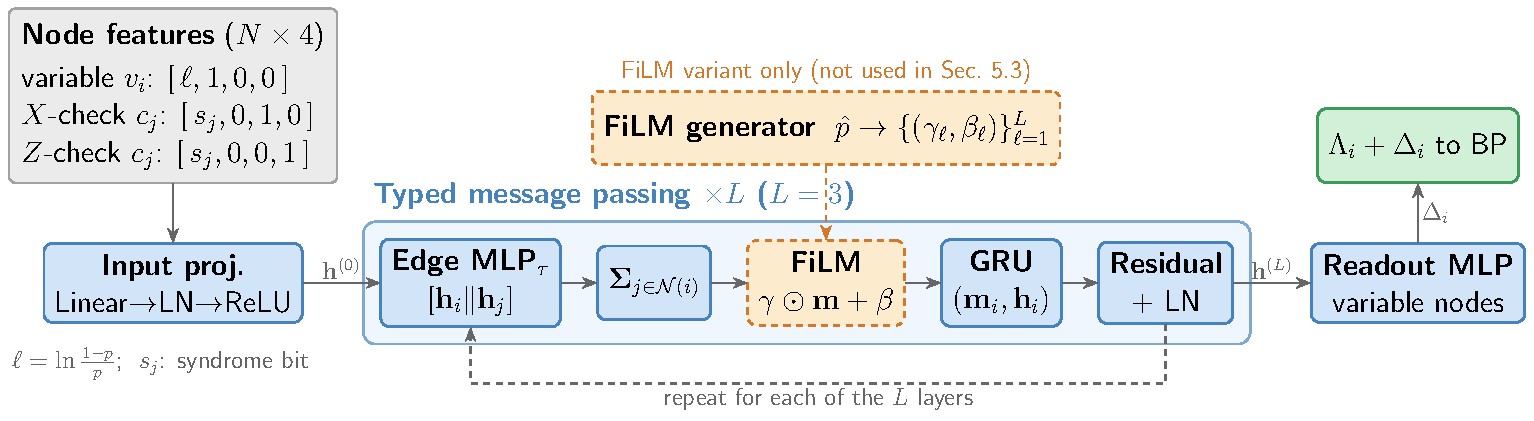
\includegraphics[width=\textwidth]{fig_tannergnn_arch}
\caption{\textsc{TannerGNN} architecture. Variable and check nodes
         exchange typed messages over $L=3$ layers via edge-type-specific
         MLPs; a GRU update aggregates messages at each node. FiLM
         modulation (not shown) scales hidden activations with
         syndrome-derived conditioning at each layer.}
\label{fig:tannergnn_arch}
\end{figure*}

\begin{remark}[Architectural limitation under biased noise]
The current implementation applies the same scalar $\Delta_i$ to
both $\llr_{z,i}$ and $\llr_{x,i}$, and computes GNN input
features from their average. Under $\eta = 20$, $\llr_{z,i}$
and $\llr_{x,i}$ differ substantially (factor $\approx 1.7$ in
LLR magnitude at $p=0.04$), so a single correction cannot
simultaneously be optimal for both error types. Separate $Z$- and
$X$-readout heads provide a direct way to remove this coupling and should
be tested under the same biased-noise conditions.
\end{remark}

\subsection{FiLM conditioning}\label{sec:film}

Feature-wise Linear Modulation (FiLM)~\cite{Perez2018FiLM} conditions
each GNN layer on an external context. A small generator network maps
the syndrome-weight estimate
$\phat = \|\synd\|_1 / (m_x + m_z)$ to per-layer affine
parameters $(\gamma^{(\ell)}, \beta^{(\ell)}) = \mathrm{FiLMGen}(\phat)$,
modulating hidden activations as
$\tilde{\bvec{h}}^{(\ell)} = \gamma^{(\ell)} \odot \bvec{h}^{(\ell)} + \beta^{(\ell)}$.
This conditioning pathway is designed to let a single model respond to
global changes in the noise level without retraining. It should not be
confused with spatial calibration: $\phat$ is one scalar shared by the
entire graph and therefore contains no direct per-qubit reliability
information. Section~\ref{sec:invariance} establishes a narrower result:
uniform rescaling of the channel prior cannot change the hard decisions
of the underlying unclipped min-sum BP decoder. That invariance does not,
by itself, imply that a GNN cannot use a global scalar as contextual
information.

\subsection{Neural BP and interleaved pipeline}\label{sec:neuralbp}

Differentiable BP generalises~\eqref{eq:vtc}--\eqref{eq:ctv} with
learnable per-iteration scaling weights $w_\mathrm{ch}^{(t)},
w_\mathrm{vtc}^{(t)}, w_\mathrm{ctv}^{(t)} = \mathrm{softplus}(w_\mathrm{raw}^{(t)})$
(softplus ensures positivity; $w_\mathrm{raw}=0$ at initialisation
gives $w \approx \ln 2 \approx 0.693$, recovering near-standard BP).

\begin{algorithm}[t]
\DontPrintSemicolon
\SetAlgoLined
\caption{Interleaved GNN-BP Decoding}\label{alg:interleaved}
\KwIn{$\synd$, channel LLR $\llr$, noise estimate $\phat$}
\KwOut{Error estimate $\ehat$}
$(\gamma,\beta) \leftarrow \mathrm{FiLMGen}(\phat)$\tcp*{Conditioning}
$\Delta^{(1)} \leftarrow \textsc{TannerGNN}(\llr, \synd, \gamma, \beta)$\;
$\llr' \leftarrow \llr + \Delta^{(1)}$\tcp*{Prior correction}
$\llr_\mathrm{mid} \leftarrow \mathrm{NeuralBP}(\llr', \Hmat, T_1)$\;
$p_i^\mathrm{mid} \leftarrow \sigma(-\llr_{\mathrm{mid},i})\;\forall i$\;
$\Delta^{(2)} \leftarrow \textsc{TannerGNN}(\llr_\mathrm{mid}, p^\mathrm{mid}, \synd, \gamma, \beta)$\;
$\llr'' \leftarrow \llr_\mathrm{mid} + \Delta^{(2)}$\tcp*{Mid correction}
$\llr_\mathrm{final} \leftarrow \mathrm{NeuralBP}(\llr'', \Hmat, T_2)$\;
$\hat{e}_i \leftarrow \mathbbm{1}[\llr_{\mathrm{final},i} < 0]\;\forall i$\;
\Return{$\ehat$}
\end{algorithm}

Algorithm~\ref{alg:interleaved} gives the interleaved pipeline.
The GNN intervenes twice: before BP to correct channel priors, and
after $T_1$ iterations using the intermediate posterior information.
Qubits with $p_i^\mathrm{mid} \approx 0.5$ have low posterior
confidence and can receive a second learned correction. Both correction
stages are trained jointly through the differentiable BP unroll.

\begin{figure*}[t]
\centering
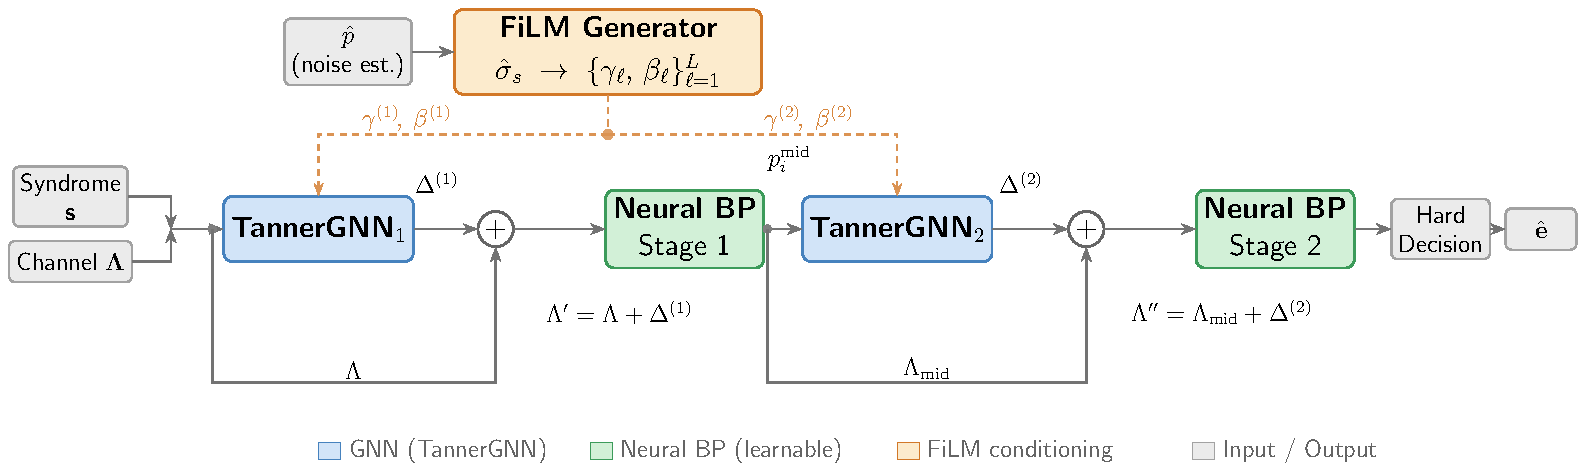
\includegraphics[width=\textwidth]{fig_interleaved_pipeline}
\caption{Interleaved GNN-BP pipeline. The GNN applies two successive
         LLR corrections: one before BP initialisation and one after
         $T_1$ iterations, using the mid-decoding posterior as an
         additional input. Both stages are trained end-to-end through
         the BP unroll.}
\label{fig:interleaved_pipeline}
\end{figure*}

\subsection{Training}\label{sec:training}

\begin{table}[t]
\centering
\caption{Architecture and training hyperparameters.}
\label{tab:hparams}
\resizebox{\columnwidth}{!}{%
\begin{tabular}{@{}ll@{}}
\toprule
\multicolumn{2}{@{}l}{\textit{GNN Architecture}} \\
\midrule
Hidden dimension $d_h$          & 64 \\
Message-passing layers $L$      & 3 \\
Edge types                      & 2 ($\Hmat_x$, $\Hmat_z$) \\
Node update                     & GRU \\
Node feature dim.               & 4 \\
FiLM conditioning               & 1 (scalar $\phat$) \\
Parameters                      & \makecell[l]{GNN-BP: 154k\\FiLM: 183k\\Interleaved: 183k} \\
\midrule
\multicolumn{2}{@{}l}{\textit{Training}} \\
\midrule
Optimizer                       & AdamW \\
Learning rate                   & $10^{-4}$ \\
Weight decay                    & $10^{-4}$ \\
Schedule                        & Cosine + 2-epoch warmup \\
Batch size                      & 16 \\
Focal loss $(\alpha,\gamma)$    & $(0.25,2.0)$ \\
Syndrome loss weight            & $0.1$ \\
BP iters (training / eval)      & 10 (flooding) / 100 \\
Best epoch                      & \makecell[l]{GNN-BP: 5 / 17\\FiLM: 18\\Interleaved: 1} \\
\midrule
\multicolumn{2}{@{}l}{\textit{Reference BP-OSD baseline}} \\
\midrule
\texttt{bp\_method}             & \texttt{ms} (min-sum) \\
\texttt{ms\_scaling\_factor}    & $0.8$ \\
\texttt{schedule}               & \texttt{serial} (layered) \\
\texttt{max\_iter}              & 100 \\
OSD (where used)                & \texttt{osd\_cs}, order 10 \\
\bottomrule
\end{tabular}}
\end{table}

Training uses focal loss~\cite{Lin2017Focal} with $\alpha=0.25$,
$\gamma=2.0$ for class-imbalanced qubit errors, together with a syndrome
consistency term. The noise range is experiment dependent; in particular,
the positive held-out result of Sec.~\ref{sec:gnn_positive} uses training
rates $p\in[0.02,0.03]$. \pending{Reconcile this with the earlier training
configuration $p\sim\mathrm{Uniform}[0.01,0.10]$ and report the data
range, number of samples per epoch, and checkpoint-selection rule for
each model variant.} Key hyperparameters are summarized in
Table~\ref{tab:hparams}.

% ============================================================
%  IV. EXPERIMENTAL SETUP
% ============================================================
\section{Experimental Setup}\label{sec:setup}

\begin{figure*}[t]
\centering
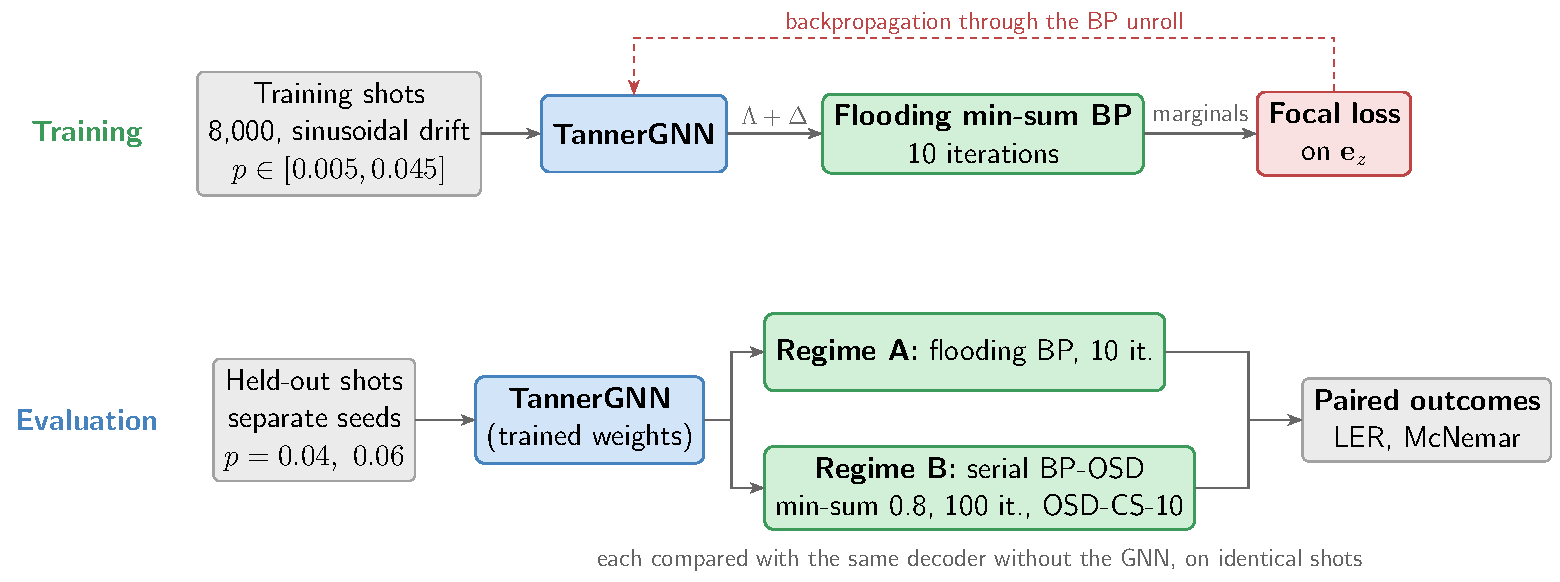
\includegraphics[width=\textwidth]{fig_experimental_pipeline}
\caption{Experimental evaluation pipeline. Syndromes are sampled under
         static or drift noise models; each decoder receives identical
         syndrome batches to enable McNemar paired testing. Oracle
         experiments substitute true per-qubit rates for the uniform
         mean prior.}
\label{fig:experimental_pipeline}
\end{figure*}

\subsection{Evaluation regimes}\label{sec:regimes}

Two distinct evaluation regimes are used throughout this paper,
and the distinction is central to interpreting the results:

\textbf{Regime A (training-aligned baseline):} The GNN is evaluated
against flooding BP, the base decoder used during training. This
comparison isolates the gain relative to the decoder represented in the
training computation graph.

\textbf{Regime B (stronger classical baseline):} The same learned
correction is evaluated with the serial-schedule min-sum BP-OSD reference
configuration. This tests whether the correction also improves the
stronger classical decoder considered here; Sec.~\ref{sec:mismatch}
shows that it does not in the tested regime.

Unless otherwise stated, all experiments use $Z$-biased noise with
$\eta = 20$.

\subsection{Statistical protocol}

For absolute LER comparisons we treat operating points with fewer than
100 observed logical-error events as preliminary; this is a reporting
heuristic rather than a formal power calculation. Decoder pairs are
evaluated on \emph{identical} syndrome samples, enabling paired
McNemar tests~\cite{McNemar1947}. We report Wilson score 95\% confidence
intervals for LER estimates.

Random seeds are fixed at $s=42$ for syndrome generation and $s+999$ for
validation splits. Unless otherwise stated, the reported learned-decoder
result is based on a single training seed; its confidence interval and
McNemar test therefore quantify test-set sampling uncertainty conditional
on that trained checkpoint, not training-to-training variability. All
training and evaluation used CPU only; no GPU was available for this work.
Representative per-epoch training times are $\sim\!17$\,s
(154k-parameter GNN-BP) and $\sim\!37$\,s (183k-parameter
interleaved model).

% ============================================================
%  V. RESULTS
% ============================================================
\section{Results}\label{sec:results}

\subsection{Decoder configuration sensitivity}\label{sec:baseline}

Before presenting the GNN results, we quantify the sensitivity of the
classical baseline to decoder configuration. This sensitivity sets the
scale against which the learned-decoder results must be interpreted.

\begin{table*}[t]
\centering
\caption{Effect of BP-OSD configuration on $\code{288}{12}{18}$,
         $p=0.04$, $\eta=20$, 5{,}000 identical shots. CIs in brackets.}
\label{tab:smoking_gun}
\begin{tabular}{@{}llllcc@{}}
\toprule
Config & Schedule & Method & Iter & LER & Errors \\
\midrule
Original BP     & parallel & prod-sum & 30  & 0.0506 [0.045,0.057] & 253 \\
Reference BP    & serial   & ms(0.8)  & 100 & 0.0014 [0.001,0.003] &   7 \\
Original BP-OSD & parallel & prod-sum & 30  & 0.0346 [0.030,0.040] & 173 \\
Ref.\ BP-OSD    & serial   & ms(0.8)  & 100 & 0.0002 [0.000,0.001] &   1 \\
\bottomrule
\end{tabular}
\end{table*}

Table~\ref{tab:smoking_gun} illustrates how strongly decoder
configuration changes the finite-length result. In the 5{,}000-shot
pilot, the original parallel product-sum BP-OSD configuration reduces
LER from $0.0506$ to $0.0346$ relative to the corresponding plain BP,
but remains far worse than the serial min-sum configurations. The
reference serial min-sum BP-OSD produces only one logical error in this
sample, so the value $0.0002$ should be interpreted as a preliminary
estimate rather than a precisely resolved LER.

A separate $N=100{,}000$-shot experiment is shown in
Fig.~\ref{fig:baseline_decomp}. In that experiment, changing to the
serial schedule and then adding OSD-CS-10 yields an overall
approximately $40\times$ reduction relative to the flooding comparator.
\pending{State the exact BP method, scaling factor, iteration count, and
stopping rule for the 100k flooding comparator. These must match the
serial configuration except for the factor being isolated; otherwise the
$6.7\times$ schedule decomposition is confounded.}

\begin{figure}[t]
\centering
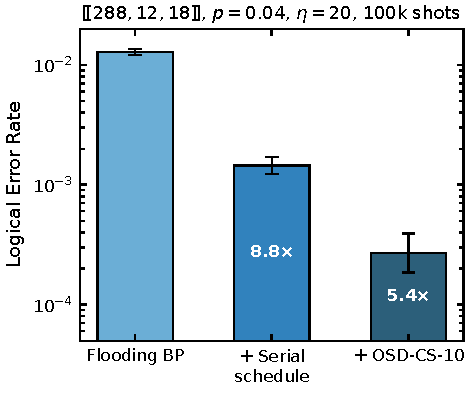
\includegraphics[width=\columnwidth]{fig_F1_baseline_decomp}
\caption{Baseline decomposition on $\code{288}{12}{18}$, $p=0.04$,
         $\eta=20$, 100k shots. The figure is intended to isolate the
         effect of serial scheduling and subsequent OSD-CS-10; the exact
         flooding-BP comparator configuration must be reported in the
         text before the multiplicative factors are interpreted causally.}
\label{fig:baseline_decomp}
\end{figure}

These data do not identify a universally optimal configuration. They do
show that schedule, update rule, iteration budget, and post-processing
can dominate the measured finite-length LER. Learned-decoder comparisons
must therefore specify and control these parameters.

\subsection{Uniform-prior scaling invariance of min-sum BP}\label{sec:invariance}

\begin{proposition}[Uniform positive-scaling invariance]\label{prop:invariance}
Consider separate-CSS min-sum BP with no message clipping or offset. If
all channel LLRs in one CSS component are multiplied by the same factor
$a>0$, then every BP message and posterior LLR is multiplied by $a$ at
every iteration. Consequently, all hard decisions are unchanged.
\end{proposition}

\begin{proof}
At initialization, each variable-to-check message is proportional to the
corresponding channel LLR and therefore scales by $a$. Assume all
variable-to-check messages at iteration $t$ have scaled by $a$. The
syndrome factor $(-1)^{s_j}$ in Eq.~\eqref{eq:ctv} is unchanged, the sign
of every message is unchanged because $a>0$, and
$\min_i a|x_i|=a\min_i|x_i|$. Hence every check-to-variable message also
scales by $a$. Equation~\eqref{eq:vtc} then shows that the next
variable-to-check messages scale by $a$. Induction establishes the claim
for all iterations and for the final posterior LLRs.
\end{proof}

For a uniform channel prior, replacing a common positive LLR $\Lambda$
by another positive value $\Lambda'$ is equivalent to the scaling
$a=\Lambda'/\Lambda$. The proposition explains why changing only the assumed uniform physical
error rate cannot change hard decisions of ideal min-sum BP. Clipping, offsets, damping rules that depend on
magnitude, non-uniform priors, or sum-product updates can break the exact
scaling argument.

We observed the expected invariance in the implemented decoder:
$1{,}740/1{,}740$ bit-identical outputs when changing the assumed prior
from $p=0.015$ to $p=0.0286$ on $\code{288}{12}{18}$, and
$1{,}000/1{,}000$ bit-identical outputs for $p=0.04$ versus $p=0.02$ in
the tested min-sum setting. The same 1{,}000-shot test was also identical
for the tested sum-product configuration; because Proposition~\ref{prop:invariance}
does not apply to the tanh nonlinearity, we report that observation as
empirical rather than structural.

\begin{remark}[What the proposition does and does not imply]
The result applies to the BP pathway when adaptivity enters only by
changing a uniform channel-prior magnitude. It does \emph{not} establish
that a global conditioning scalar is information-theoretically useless
to a GNN: a learned model could combine a global noise estimate with
local syndrome structure and change its nonlinear decision rule. The experiments below test a narrower hypothesis: spatially resolved
per-qubit calibration can change the relative reliabilities seen by the
decoder, whereas a single graph-wide scalar cannot provide that spatial
information.
\end{remark}

\subsection{GNN improvement over flooding BP}\label{sec:gnn_positive}

We evaluated the GNN against flooding BP---the decoder it was
trained against---on 8{,}000 held-out syndromes.

\begin{table}[t]
\centering
\caption{GNN-BP vs.\ flooding BP on $\code{72}{12}{6}$, $\eta=20$,
         8{,}000 held-out test syndromes. GNN trained for 20 epochs
         on separate 8{,}000 training syndromes at $p\in[0.02,0.03]$.
         Best checkpoint at epoch 5 by validation LER.}
\label{tab:gnn_flooding}
\resizebox{\columnwidth}{!}{%
\begin{tabular}{@{}lcccc@{}}
\toprule
 & Flooding BP & GNN-BP & $n_{10}$ / $n_{01}$ & McNemar $p$ \\
\midrule
$p=0.04$, ep. 5 & 0.0990 & 0.0838 & 170 / 48 & $\approx 0$ \\
$p=0.04$, ep. 1 & 0.0990 & 0.0975 & 91 / 79  & 0.399 \\
\bottomrule
\end{tabular}}
\end{table}

Table~\ref{tab:gnn_flooding} gives the primary learned-decoder result.
At the epoch-5 checkpoint, GNN-BP reduces LER by $15.4\%$ relative to
flooding BP on 8{,}000 held-out syndromes at $p=0.04$
($n_{10}=170$, $n_{01}=48$, McNemar $\chi^2=67.16$,
$p<10^{-15}$). The test point lies outside the training range
$p\in[0.02,0.03]$, so the result demonstrates transfer to a higher
physical error rate for this checkpoint. Because only one training seed
is reported, we do not interpret the paired test as evidence for
training-to-training reproducibility. A gradient audit found non-zero
signal through the network (input-to-readout gradient ratio $0.22$) and
non-trivial LLR corrections (mean $|\Delta_i|=0.854$).

A fixed-dataset capacity test provides an additional diagnostic: a GNN
trained on 1{,}000 fixed syndromes for 50 epochs achieved a $14\%$ LER
reduction on those same syndromes (McNemar $p=0.004$, $n_{10}=17$,
$n_{01}=3$). This experiment tests the ability of the architecture and
optimizer to fit the supplied examples; it is not a generalization
result. The interleaved model reached its best validation checkpoint at
epoch 1 and did not train successfully, so no performance conclusion
about that architecture is drawn from the current run (see Limitations).

\begin{figure}[t]
\centering
\includegraphics[width=\columnwidth]{fig_F5_interleaved_training}
\caption{Interleaved model training curves (183k parameters).
         The best validation checkpoint occurs at epoch~1 and the
         validation loss increases thereafter. The current run does
         not provide a trained interleaved decoder for comparison.}
\label{fig:interleaved_training}
\end{figure}

\subsection{Training/evaluation baseline mismatch}\label{sec:mismatch}

Although the GNN improves flooding BP, the same correction does not
improve the serial min-sum BP-OSD reference configuration. Note that Tables~\ref{tab:gnn_flooding}
and~\ref{tab:gnn_null} report different evaluation regimes
(Regime~A and Regime~B of Sec.~\ref{sec:regimes}) on different
syndrome sets, and their LER values are not directly comparable:

\begin{table}[t]
\centering
\caption{GNN-BP vs.\ serial BP-OSD on $\code{72}{12}{6}$, $\eta=20$,
         8{,}000 shots. Decoders evaluated on identical syndromes.}
\label{tab:gnn_null}
\resizebox{\columnwidth}{!}{%
\begin{tabular}{@{}lcccl@{}}
\toprule
$p$ & Serial BP-OSD & GNN+OSD & $p_\mathrm{McN}$ & Verdict \\
\midrule
0.020 & 0.0046 & 0.0050 & 0.68 & tie \\
0.030 & 0.0377 & 0.0399 & 0.63 & tie \\
0.040 & 0.0831 & 0.0876 & 0.033 & GNN \emph{worse} \\
0.050 & 0.1515 & 0.1555 & $3.6\!\times\!10^{-5}$ & GNN \emph{worse} \\
\bottomrule
\end{tabular}}
\end{table}

\begin{figure}[t]
\centering
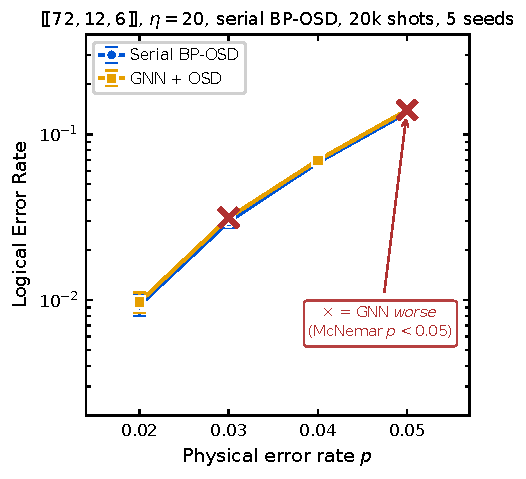
\includegraphics[width=\columnwidth]{fig_F4_phase4_ler}
\caption{GNN+OSD vs.\ serial BP-OSD LER on $\code{72}{12}{6}$,
         $\eta=20$, 8{,}000 shots. Red $\times$ marks operating points
         where GNN is statistically worse (McNemar $p<0.05$).
         Wilson 95\% CI error bars.}
\label{fig:gnn_null_curve}
\end{figure}

Table~\ref{tab:gnn_null} and Fig.~\ref{fig:gnn_null_curve} show that
the GNN-corrected decoder is statistically indistinguishable from serial
BP-OSD at the two lower error rates and significantly \emph{worse} at
the two higher rates. The same checkpoint improves flooding BP, so these
data show that the learned correction does not transfer unchanged to the
stronger decoder.

The experiment establishes a transfer failure, but it does not by itself
identify the residual-failure mechanism. The GNN was optimized through a
10-iteration flooding-BP computation graph and is then inserted ahead of
a decoder with a different schedule, iteration budget, and OSD
post-processing. The experiment therefore does not establish that LLR
corrections learned through the flooding-BP computation graph remain
useful after the schedule, iteration budget, and post-processing are
changed. At the same time,
claims that the two decoders fail on ``structurally different'' trapping
sets require an explicit paired failure-overlap or trapping-set analysis,
which is not included here. \pending{If available, add the Jaccard/overlap
statistics of the two failure sets and classify representative failures;
otherwise keep the explanation at the level of training/evaluation
mismatch.} Training directly against the target decoder, or against a
differentiable surrogate of its post-processing stage, remains the
appropriate test of whether learned augmentation can improve BP-OSD.

\subsection{Per-qubit calibration gap}\label{sec:oraclegap}

Under spatially non-uniform per-qubit noise ($p_i \sim
\mathrm{LogNormal}(\log p_\mathrm{mean}, \sigma)$, fresh per shot),
a decoder knowing the true per-qubit rates substantially outperforms
a mean-prior decoder.

\begin{figure}[t]
\centering
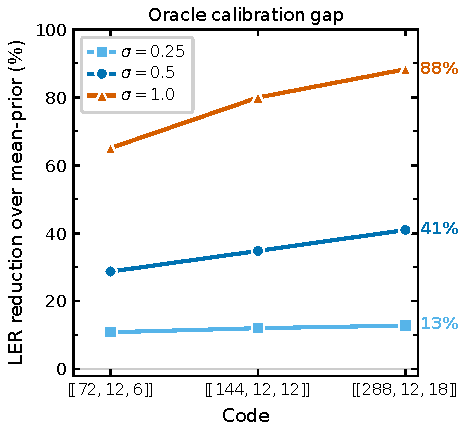
\includegraphics[width=\columnwidth]{fig_F2_oracle_vs_distance}
\caption{Oracle calibration gap (percentage LER reduction from
         per-qubit vs.\ mean-prior BP-OSD) at $\sigma=1.0$,
         50k shots ($\code{72}{12}{6}$, $\code{144}{12}{12}$)
         and 30k shots ($\code{288}{12}{18}$).
         Operating points: $p=0.04$, $0.06$, $0.07$ respectively;
         cross-code comparisons are partially confounded by the
         differing operating points.}
\label{fig:oracle_gap}
\end{figure}

\begin{table*}[t]
\centering
\caption{Oracle gap: percentage LER reduction from per-qubit
         over mean-prior BP-OSD. All McNemar $p \ll 10^{-3}$.
         Parenthetical counts are mean-prior error events.}
\label{tab:oracle}
\begin{tabular}{@{}lccc@{}}
\toprule
Code ($d$) & $\sigma=0.25$ & $\sigma=0.5$ & $\sigma=1.0$ \\
\midrule
$\code{72}{12}{6}$   (6)  & $+11\%$ (3457) & $+30\%$ (3420) & $+66\%$ (2988) \\
$\code{144}{12}{12}$ (12) & $+16\%$ (276)  & $+38\%$ (268)  & $+74\%$ (2604) \\
$\code{288}{12}{18}$ (18) & $+18\%$ (922)  & $+48\%$ (524)  & $+87\%$ (1750) \\
\bottomrule
\end{tabular}
\end{table*}

Table~\ref{tab:oracle} and Fig.~\ref{fig:oracle_gap} show a clear
increase with noise contrast $\sigma$ for each tested code. The reported
percentage reduction is also larger for the larger-code rows, reaching
$87\%$ on $\code{288}{12}{18}$ at $\sigma=1.0$; however, the physical
error rate is changed across codes ($p=0.04$, $0.06$, and $0.07$).
Consequently, these data do not isolate code distance as the cause of
the cross-code trend.

This experiment isolates the value of synthetic per-qubit rate side
information; it does not require machine learning. We use the true-rate
decoder as an \emph{oracle reference}, not as a formal upper bound on all
possible decoders. The comparison quantifies how much the tested BP-OSD
implementation can benefit when the realized per-qubit rates are
revealed. The gap is \emph{not}
recoverable from a single syndrome shot under i.i.d.\ per-qubit
noise: with a fresh field redrawn every shot, the uniform mean
prior is Bayes-optimal within the class of estimators that observe
only the syndrome, so no syndrome-conditioned GNN can do better
than the mean prior in this regime. A GNN that attempts to estimate
per-qubit rates from a single syndrome is significantly
\emph{worse} than the mean prior at $\sigma=1.0$ (GNN LER = 0.069
vs.\ mean LER = 0.064, McNemar $p = 2.7\times10^{-4}$)---not
because the architecture is broken, but because the task is
information-theoretically infeasible.

\subsection{Drift adaptation}\label{sec:drift}

Under persistent OU drift ($\sigma=1.0$, $W=32$-round window,
$\code{72}{12}{6}$, $p=0.04$, 6{,}000 shots), the GNN beats
stale calibration only at the highest tested drift volatility.

\begin{table*}[t]
\centering
\caption{LER under per-qubit OU drift by volatility (vol).
         ``Empir'': non-learned per-qubit frequency estimator.}
\label{tab:drift}
\begin{tabular}{@{}lccccl@{}}
\toprule
vol & Oracle & Stale & Empir & GNN & Verdict \\
\midrule
0.00 & 0.033 & 0.033 & 0.057 & 0.064 & GNN worse, $p=5\!\times\!10^{-36}$ \\
0.10 & 0.031 & 0.038 & 0.057 & 0.067 & GNN worse, $p=8\!\times\!10^{-30}$ \\
0.35 & 0.005 & 0.027 & 0.038 & 0.050 & GNN worse, $p=5\!\times\!10^{-19}$ \\
0.50 & 0.004 & 0.052 & 0.035 & \textbf{0.044} & GNN beats stale, $p=0.005$ \\
\bottomrule
\end{tabular}
\end{table*}

\begin{figure}[t]
\centering
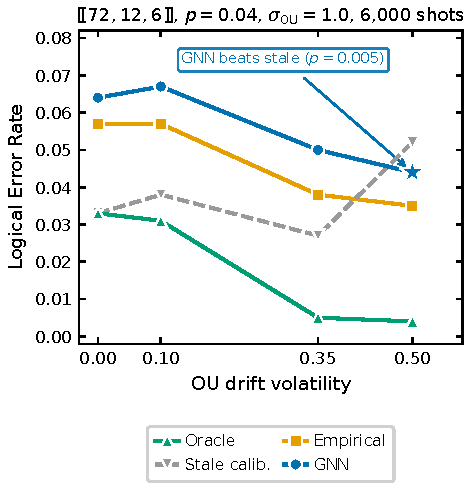
\includegraphics[width=\columnwidth]{fig_F3_drift_adaptation}
\caption{LER vs.\ OU drift volatility for four decoder configurations
         on $\code{72}{12}{6}$, $p=0.04$, $\sigma_\mathrm{OU}=1.0$, 6{,}000 shots.
         Star marks the single operating point (vol$=0.5$) where GNN
         beats stale calibration ($p=0.005$); GNN is beaten by the
         empirical frequency estimator at every volatility level.}
\label{fig:drift_curve}
\end{figure}

Table~\ref{tab:drift} and Fig.~\ref{fig:drift_curve} show that the GNN beats stale calibration
at vol$=0.5$ ($p=0.005$, 158 vs.\ 111 discordant pairs), but
is beaten by the non-learned empirical frequency estimator at
every volatility level (GNN vs.\ empir: $p = 2.7\times10^{-8}$
at vol$=0.5$, GNN worse). Under independent per-qubit drift,
direct per-qubit syndrome frequency counting captures most of
the available signal, leaving little room for a learned estimator.
Whether spatial correlation structure between qubits would shift
this result is an open question.

\subsection{Circuit-level evaluation}\label{sec:circuit}

\pending{Specify the complete circuit-level noise model: syndrome
extraction circuit, number of data/check qubits, gate/reset/measurement
error channels and rates, treatment of bias/Y errors, detector
construction, and BP-OSD configuration. Without these details the
circuit-level result is not reproducible.}

\begin{table}[t]
\centering
\caption{Circuit-level oracle gap on $\code{72}{12}{6}$, 6 rounds,
         $\eta=20$, 5{,}000 shots per point (preliminary,
         $N=5{,}000$ shots, underpowered).}
\label{tab:circuit}
\resizebox{\columnwidth}{!}{%
\begin{tabular}{@{}lcccc@{}}
\toprule
$p_\mathrm{mean}$ & Mean LER & Oracle LER & Discordant & McNemar $p$ \\
\midrule
0.001 & 0.272 & 0.270 & 3 & 0.25 \\
0.003 & 0.335 & 0.335 & 8 & 1.00 \\
\bottomrule
\end{tabular}}
\end{table}

\begin{figure}[t]
\centering
\includegraphics[width=\columnwidth]{fig_F6_circuit_null}
\caption{Circuit-level oracle gap on $\code{72}{12}{6}$, 6 rounds,
         $\eta=20$, 5{,}000 shots. No statistically detectable
         difference between mean-prior and per-qubit-oracle BP-OSD
         at either operating point (McNemar $p \geq 0.25$; 3 and 8
         discordant pairs---underpowered, see text).}
\label{fig:circuit_null}
\end{figure}

Table~\ref{tab:circuit} and Fig.~\ref{fig:circuit_null} show no
statistically detectable oracle gap at circuit level. With only 3
and 8 discordant pairs at the two tested operating points, however,
McNemar's test cannot distinguish a true zero gap from a gap of up
to approximately $1.5\%$ LER---consistent with the code-capacity
oracle gap at low contrast. The present sample cannot distinguish between negligible prior
sensitivity and a nonzero gap below the resolution of the experiment. Higher shot counts (targeting $\geq 100$ discordant
pairs) are required to distinguish these cases.
The two prior assignments are nevertheless numerically distinct: 86\%
of fault mechanisms change rank by more than 50 positions and the
per-mechanism probability ratios span $0.25\times$--$5.1\times$. The
DEM contains 3{,}821 fault mechanisms and 360 detectors, suggesting that
many fault mechanisms map to the same detector information. This
high degeneracy is a plausible explanation for the weak prior
sensitivity, but the present experiment does not isolate it causally.
An ablation that changes DEM degeneracy while holding the prior mismatch
fixed would be required for that conclusion.

Thus, the circuit-level experiment is currently a null result with
insufficient statistical resolution; it does not establish that
calibration side information is irrelevant at circuit level.

% ============================================================
%  VI. DISCUSSION
% ============================================================
\section{Discussion}\label{sec:discussion}

\subsection{The GNN's role and its limits}

\textsc{TannerGNN} achieves a $15.4\%$ LER reduction over the flooding
BP decoder used in its training loop. The paired held-out test supports a
real difference for this trained checkpoint, while gradient diagnostics
show that the network produces non-trivial corrections. Robustness to
training initialization has not yet been measured, so we do not treat the
single-seed result as a reproducibility claim.

The Regime-B result is also informative: the learned correction does
not transfer automatically to serial BP-OSD. This is consistent with the
training/evaluation mismatch, but the residual failure sets have not yet
been characterized well enough to claim a trapping-set mechanism.
Training against BP-OSD directly is complicated by the non-differentiable
OSD stage; differentiable surrogates, distillation, or training on the
residual failures of the target decoder are possible alternatives.

\subsection{Benchmark design implications}

The baseline experiments identify two reporting requirements for learned
QLDPC decoders. First, BP-OSD schedule, update rule, iteration count, and
OSD configuration must be stated explicitly because they can change LER
by more than two orders of magnitude on the same code. Table~\ref{tab:hparams}
records these settings for the present study.

Second, the training and evaluation decoders must be distinguished. An
LLR correction learned through flooding BP need not remain beneficial
when the schedule, iteration count, and OSD stage are changed. Comparisons
across such decoder configurations should identify the mismatch rather
than treating all BP-based baselines as equivalent.

\subsection{Comparison with prior work}\label{sec:priorwork}

Astra~\cite{Maan2025MLBP} uses a learned Tanner-graph message-passing
decoder and reports BB-code performance competitive with, and in several
settings better than, BP-OSD under code-capacity depolarizing noise. This
places our $15.4\%$ flooding-BP gain in context: improvement over plain BP
is not, by itself, the main novelty. Our contribution is instead the
controlled comparison showing how that gain changes when the baseline
and side information are strengthened.

Gong et al.~\cite{Gong2024GNN} interleave differentiable BP stages with
GNN corrections on the same sparse graph and show error-floor
improvements over several post-processing approaches. Our interleaved
variant follows the same broad design principle, but the checkpoint
reported here does not train successfully. We therefore do not claim a
competitive result for that architecture.

Recent circuit-level work on BB codes also reports neural decoders that
can outperform BP-OSD on the $\code{72}{12}{6}$ code while retaining a
runtime advantage, although scaling to $\code{144}{12}{12}$ remains more
challenging~\cite{Blue2026MLBB}. This comparison reinforces the need to evaluate learned decoders against
a fully specified competitive non-learned baseline, not only against
flooding BP.

Stein et al.~\cite{Stein2026FiLM} condition a neural QEC decoder on
spatially resolved hardware calibration data using FiLM and evaluate on
IBM repetition-code experiments. Their conditioning signal is per-qubit
and calibration-derived, unlike the single scalar $\phat$ used in our
initial model. This distinction is consistent with the oracle experiments
of Sec.~\ref{sec:oraclegap}, which motivate spatial rather than purely
global conditioning.
\subsection{Towards spatially-resolved conditioning}\label{sec:srcf}

The oracle-gap experiment (Sec.~\ref{sec:oraclegap}) shows that
per-qubit rate side information can materially improve the tested
BP-OSD decoder. Because operating point and code size co-vary, the
current data do not establish how this value scales with distance.
Proposition~\ref{prop:invariance} also shows that a uniform rescaling
of the min-sum BP prior cannot reproduce the effect of spatially varying
reliabilities. These results motivate testing spatially resolved FiLM
(SRCF), in which per-qubit parameters $(\gamma_i, \beta_i)$ are
conditioned on persistent hardware calibration data rather than on a
single graph-wide scalar. Such a decoder should be compared with the
non-learned frequency estimator of Sec.~\ref{sec:drift} and evaluated
in a circuit-level setting where the calibration signal remains
identifiable. Neither condition has been established in the present
experiments.

\subsection{Limitations}\label{sec:limitations}

\begin{enumerate}[leftmargin=*,topsep=3pt,itemsep=2pt,
                  label=(\roman*)]
\item The primary $15.4\%$ GNN result uses one training seed. Statistical
      uncertainty over independent training runs has not been measured.
\item All GNN variants were trained against 10-iteration
      flooding BP. No variant was trained against serial BP-OSD,
      which is the competitive classical baseline. Whether GNN
      augmentation of serial BP-OSD yields gains is untested.
\item GNN checkpoints exist only for $\code{72}{12}{6}$; the
      larger codes were not trained due to CPU-only compute
      constraints. The null result in Regime B should not be
      extrapolated to the larger codes.
\item The interleaved model reached its best validation checkpoint at epoch 1,
      after which the validation loss increased. The current run is therefore
      insufficient to evaluate the interleaved architecture.
\item All training and evaluation used CPU only, which limited
      hyperparameter search and training duration.
\item The single per-qubit correction $\Delta_i$ is applied to
      both $\llr_{z,i}$ and $\llr_{x,i}$, which is suboptimal
      under $\eta = 20$ biased noise; separate $Z$/$X$ readout
      heads are the recommended fix.
\item Code-capacity noise omits measurement errors, leakage,
      and correlated faults present in real circuits.
\end{enumerate}

% ============================================================
%  VII. CONCLUSION
% ============================================================
\section{Conclusion}\label{sec:conclusion}

On $\code{72}{12}{6}$, a Tanner-graph GNN trained through
10-iteration flooding BP reduces the held-out LER by $15.4\%$ at
$p=0.04$ and $\eta=20$. The same learned correction does not improve the
serial min-sum BP-OSD reference decoder and increases LER at the two
highest tested error rates. The demonstrated gain is therefore specific
to the training-aligned flooding-BP baseline; the present experiments do
not establish an improvement over competitive BB decoding more generally.

The baseline experiments show that BP schedule, update rule, iteration
budget, and OSD configuration can change finite-length LER by orders of
magnitude. These parameters must be treated as part of the decoder
specification when learned and non-learned methods are compared. We also
proved that uniform positive rescaling of the channel LLRs leaves the
hard decisions of ideal min-sum BP unchanged. A global prior magnitude
alone therefore cannot provide spatial adaptation to heterogeneous qubit
reliabilities, although a nonlinear learned model may still use a global
noise estimate as context.

The synthetic oracle experiments identify per-qubit calibration as the
more informative adaptive signal in the tested setting: revealing the
true per-qubit rates substantially improves BP-OSD under heterogeneous
noise. The current cross-code experiments do not isolate how this gain
scales with distance, and the circuit-level study does not yet have
sufficient statistical resolution. A direct next test is to condition a
learned decoder on persistent spatial calibration data and compare it
against a fully specified serial BP-OSD baseline and the non-learned
frequency estimator, using multiple training seeds and a noise model that
preserves temporal calibration structure.
\section*{Acknowledgments}

The authors thank the STAR Lab program at the University of Arizona
for facilitating this research and providing computational resources.

\section*{Data and code availability}

Source code, trained checkpoints, all datasets, and the audit scripts
that produced the findings of Secs.~\ref{sec:baseline}
and~\ref{sec:invariance} are available at
\url{https://github.com/anish-chedalla/adaptive_gnn}.
Syndrome data were generated using Stim~\cite{Gidney2021Stim}.

\bibliographystyle{quantum}
\bibliography{references}

\end{document}
